\setlength{\footskip}{8mm}

\chapter{Literature Review} 
\label{ch:literature-review}

\textit{Some intro..}

\section{Software Architecture of Autonomous Driving Vehicle}
\label{section-name-in-literature-review}

\shortciteA{sbehere16t} has split the major components of the motion control part of the autonomous driving system into three main categories as shown in Figure \ref{fig:fav_automonous}. These categories are

\begin{itemize}
	\item Perception of the external environment in which the vehicle operates
	\item Decisions and control of the vehicle motion, with respect the external environment that is perceived
	\item Vehicle platform manipulation which deals mostly with sensing, control and actuation of the Ego vehicle, with the intention of achieving desired motion.
\end {itemize}

Each category can be further broken down into several components.

\subsection{Perception}

The \textbf{sensing components} senses the states of the vehicle and the states of the environment in which the vehicle operates. The \textbf{sensor fusion component} considers multiple sources of information to construct a hypothesis about the state of the environment. The \textbf{localization component} determines the location of the vehicle with respect to a global map. The \textbf{semantic understanding component} processes the sensor input and derives meaningful information form it. The \textbf{world model component} holds the state of the external environment.

\subsection{Decision and Control}
The \textbf{trajectory generation component} repeatedly generates a set of obstacle free trajectories in the world coordinate system and pick an optimal trajectory from the set.  \textbf{Energy management components} deals with energy management of the vehicle. \textbf{Diagnosis and fault management} monitors state of the overall system and its components. \textbf{Reactive control components} are used for immediate responses to unanticipated stimuli from the environment. The \textbf{vehicle platform abstraction component} refers to a minimal model of the vehicle platform. 

\subsection{Vehicle Platform Manipulation}

The \textbf{platform stabilization components}'s task is to keep the vehicle platform in a controllable state during operation. The \textbf{trajectory execution components} are responsible for executing the trajectory generated by Decision and Control. 

\begin{figure}
	\centering
	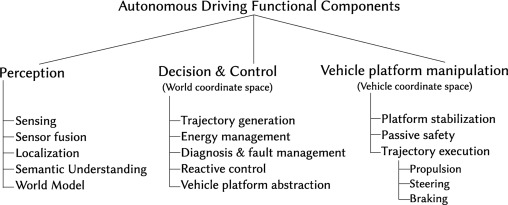
\includegraphics[width=5in]{figures/fav_autonomous_driving}
	\caption[FAV of Antonomous Driving System.]{\small 
		Functional Architecture View of Autonomous Driving System. Reprinted from work of \shortciteA{sbehere16t} }
	\label{fig:fav_automonous}
\end{figure}

\section{Coordinate Systems}
	
\subsection{Earth Centric, Earth Fixed}

The earth-centered earth-fixed (ECEF), rotates with the Earth and has its origin at the center of the Earth. Figure \ref{fig:coordinatesystem} a.

It follows the right hand coordinate system. And \shortcite{coordinatesystem} describes it as:

\begin{itemize}
	\item The origin at the center of mass of the Earth, a point close to the Earth's center of figure
	\item The Z axis on the line between the North and South Poles, with positive values increasing northward (but does not exactly coincide with the Earth's rotational axis)
	\item The X and Y axes in the plane of the Equator
	\item The X axis passing through extending from 180 degrees longitude at the Equator (negative) to 0 degrees longitude (prime meridian) at the Equator (positive)
	\item The Y axis passing through extending from 90 degrees west longitude at the Equator (negative) to 90 degrees east longitude at the Equator (positive)
\end{itemize}

\subsection{Local tangent plane}

In local tangent coordinate system, a position in earth is fixed as the origin. There are two conventions as shown in Figure \ref{fig:coordinatesystem} b.

\begin{itemize}
	\item East(x), North(y), UP(z) (ENU).
	\item North(x), East(y), Down(z) (NED), which is mostly used is aviation as the objects of interest lies before an aircraft.
\end{itemize}

\begin{figure}%
	\centering
	\subfloat[\small Earth Centric, Earth Fixed coordinate system. By Krishnavedala - Own work, CC BY-SA 3.0]{{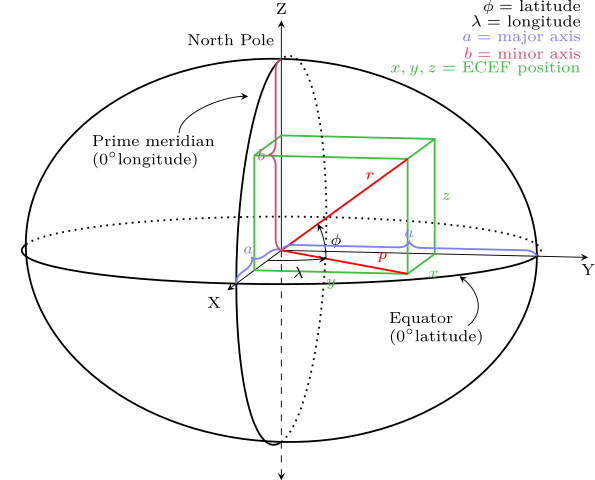
\includegraphics[width=3in]{figures/ECEF}}}%
	\subfloat[\small Local tangent plane coordinate systems]{{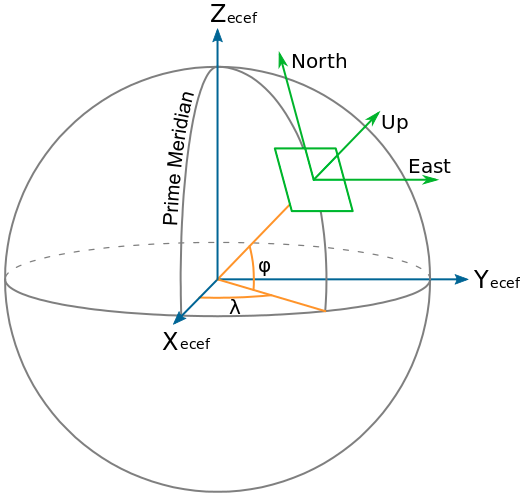
\includegraphics[width=3in]{figures/ENU_NED}}}%
	\caption[ECEF coordinate system]{\small Coordinate Systems
	}%
	\label{fig:coordinatesystem}%
\end{figure}

\subsection{Pixhawk and ROS coordinates}

Pixhawk follows NED convention, whereas ROS follows ENU convention. The conversion between these different conventions is handled automatically by MAVROS. For translate airframe related data rotation of 180° is applied about ROLL (X) axis. For local 180° rotation is applied about ROLL (X) and 90° about YAW (Z) axes.

ROS has other reference frames as described in \shortcite{rosrefframes}.

\begin{itemize}
	\item The coordinate frame called \textbf{base\_link} is rigidly attached to the mobile robot base. It can be attached in any arbitrary position or orientation.
	\item The coordinate frame called \textbf{odom} is a world-fixed frame. The pose of a robot is continuous in this frame, but it can drift over time.
	\item The coordinate frame called \textbf{map} is a world fixed frame, with its Z-axis pointing upwards. 
	\item The coordinate frame called \textbf{earth} is the origin of ECEF.
\end{itemize}

The relationship between these frames is shown in Figure \ref{fig:rosrefframes}.

\begin{figure}
	\centering
	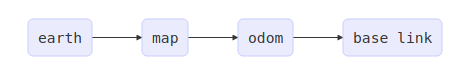
\includegraphics[width=5in]{figures/ros_rel_frames}
	\caption[FAV of Antonomous Driving System.]{\small 
	Relationship between ros frame. \shortciteA{rosrefframes} }
	\label{fig:rosrefframes}
\end{figure}

\section{Simultanious Localization and Mapping}

\shortcite{slamp1} describes SLAM problem as a process by which a mobile robot can build a map of an environment and at the same time use this map to deduce its location. In SLAM, both the trajectory of the platform and the location of all landmarks are estimated online without the need for any a priori knowledge of location.

In probabilistic SLAM, the probability distribution, 
\begin{equation} \label{eq:slam1}
P({\bf x}_{k},{\bf m}\vert {\bf Z}_{0:k},{\bf U}_{0:k},{\bf x}_{0})
\end{equation}
has to be computed at any time instance $k$. Where
\begin{itemize}
	\item ${\bf x}_k$: the state vector describing the pose of the vehicle.
	
	\item ${\bf u}_k$: the control vector, applied at time $k - 1$ to drive the vehicle to a state ${\bf x}_k$ at time $k$.
	
	\item ${\bf m}_i$: a vector describing the location of the $ith$ landmark whose true location is assumed time invariant. This is the map of the environment.
	
	\item ${\bf z}_{ik}$: an observation taken from the vehicle of the location of the $ith$ landmark at time $k$.
	
	\item ${\bf m}$: the set of all landmarks detected
	
	\item ${\bf Z}_{0:k}$: the set of all observations upto time $k$
	
	\item ${\bf U}_{0:k}$: the set of all control input upto time $k$
	
\end{itemize}

The best estimate of ${\bf x}_k$ (pose) and ${\bf m}$ (map) at any time instance $k$ would be maximizing \ref{eq:slam1}.

The \textit{observation model} describes the probability of making an observation ${\bf z}_k$ when the vehicle location and landmark locations are known and is generally described in the form
\begin{equation}
P({\bf z}_{k}\vert {\bf x}_{k},{\bf m})
\end{equation}

The\textit{ motion model} for the vehicle can be described in terms of a probability distribution on state transitions in the form
\begin{equation}
P({\bf x}_{k}\vert {\bf x}_{k-1},{\bf u}_{k})
\end{equation}

The state transition is assumed to be a Markov process which is independent of both the observations and the map. The next state ${\bf x}_k$ depends only on the immediately preceding state ${\bf x}_{k−1}$ and the applied control ${\bf u}_k$.

Now, the pose of the vehicle and map can be estimated by standard two-step recursive (sequential) prediction (time-update) correction (measurement-update) form:

\textbf{Time Update}
\begin{equation}
P({\bf x}_{k},{\bf m}\vert {\bf Z}_{0:k-1},{\bf U}_{0:k},{\bf x}_{0})= \int P({\bf x}_{k}\vert {\bf x}_{k-1},{\bf u}_{k}) \quad\times P({\bf x}_{k-1},{\bf m}\vert {\bf Z}_{0:k-1}, {\bf U}_{0:k-1},{\bf x}_{0}){\rm d}{\bf x}_{k-1}
\end{equation}

\textbf{Measurement Update}
\begin{equation}
P({\bf x}_{k},{\bf m}\vert {\bf Z}_{0:k},{\bf U}_{0:k},{\bf x}_{0}) = {P({\bf z}_{k}\vert {\bf x}_{k},{\bf m})P({\bf x}_{k}, {\bf m}\vert {\bf Z}_{0:k-1},{\bf U}_{0:k},{\bf x}_{0})\over P({\bf z}_{k}\vert {\bf Z}_{0:k-1},{\bf U}_{0:k})}
\end{equation}

An alternate way of formulating the problem would be.

If the location of the vehicle ${\bf x}_k$ is know at all times. The map can be estimated by computing
\begin{equation}
P({\bf m}\vert {\bf X}_{0:k},{\bf Z}_{0:k}, {\bf U}_{0:k})
\end{equation}
. 

If the landmark locations are known, the vehicles can be localized by computing
\begin{equation}
P({\bf x}_k\vert {\bf Z}_{0:k},{\bf U}_{0:k}, m)
\end{equation}

\section{Visual SLAM}


\FloatBarrier

